\begin{figure}[H]
  \caption{Three tiers architecture of the system}
  \label{3tiers}
  \centering
  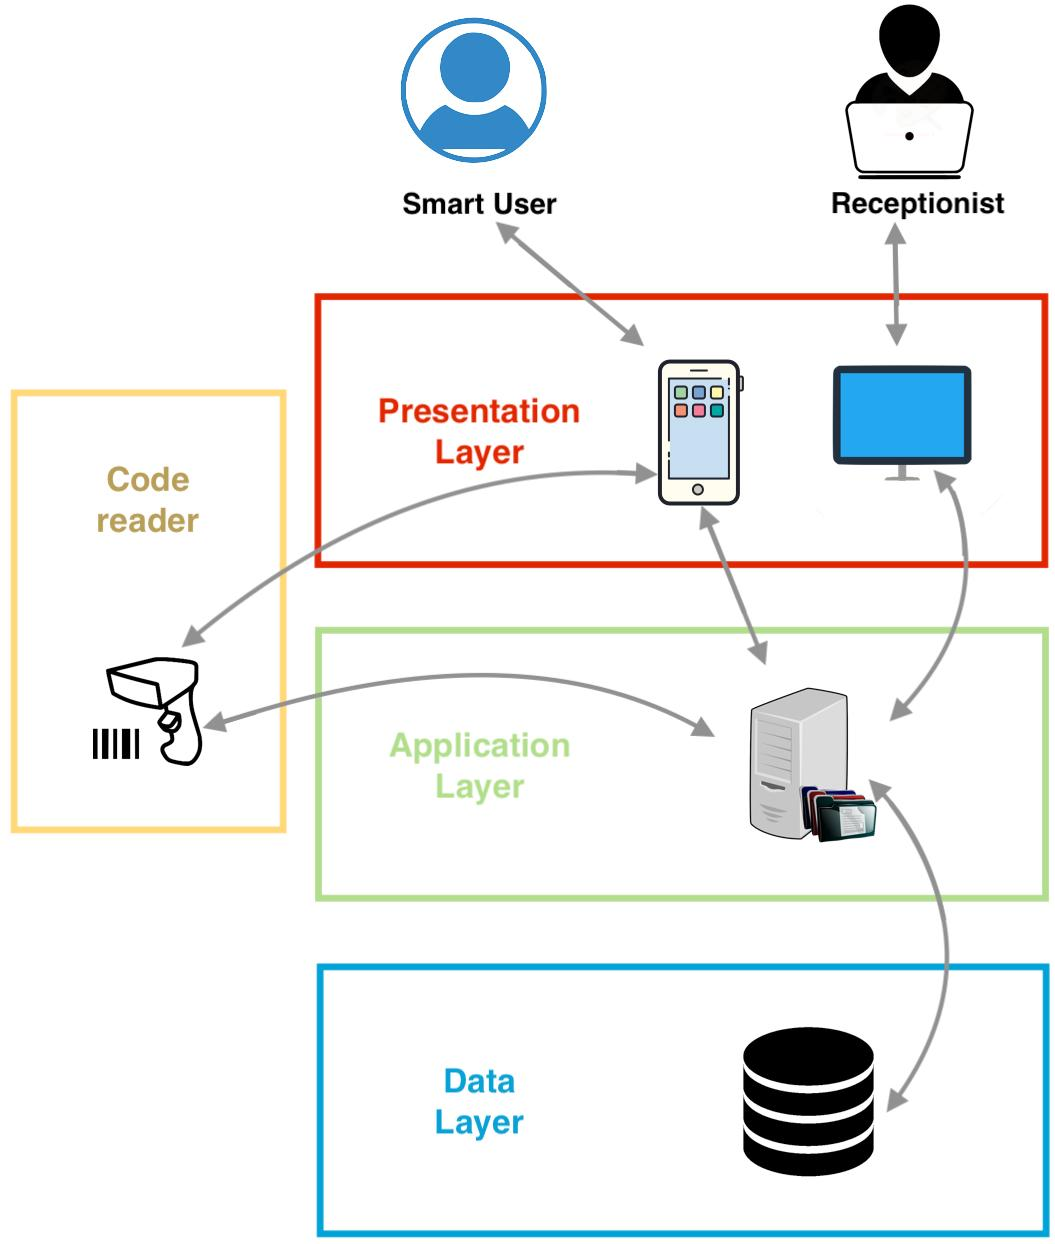
\includegraphics[scale=0.25]{diagrams/3_tiers.jpeg}

\end{figure}


\section{Overview: High-level components and their interaction}
The system is organized following the three tiers architecture. This aims to decouple logical layers in order to gurantee an horizontal scalability and a low fault tolerance.
Graphically it's shown in the figure~\ref{3tiers}.
\par


\textbf{Presentation layer}. It's the front end layer which consists of the user interface. We have two types of user interface, depending on his funcitonality: 
\begin{itemize}
\item \textbf{CLup}: It's the mobile application used by users who have a smartphone. They can manage their booking by themselves;
\item \textbf{CLup Operator}: It's the desktop application used by receptionists who act as an intermediary to manage booking of users that have only a mobilephone.
\end{itemize}

\textbf{Application layer}. It deals with the model of the system, by containing the business logic of the application. In our system it consists in a remote server to which mobile and desktop applications have to connect due to manage any bookings.

\textbf{Data layer}. It's composed by a data storage system. It includes: 

\begin{itemize}
\item User sensitive data asked during the registration process;
\item Information about user's grocery shopping;
\end{itemize}



\section{Component view}
component diagram ogni componente descritto
er diagram o class diagram specificp

-strittura
-model applicazione
-database


\section{Deployment view}
-deployment diagram

\section{Runtime view}
sequence diagrams

\section{Component interfaces}
ogni componente
app
server+db
laptop receptionist

\section{Selected architectural styles and patterns}
mvc + tier + ..

\section{Other design decisions}

security+google api

